\chapter{Lec 08 - Neural Networks II}

\section{Activation functions}
Let's consider the Perceptron artificial neuron. The output of the neuron is obtained by computing the $net$ and passing it to the step function (hard threshold). Due to the discontinuity of this function, it could be difficult to combine multiple neurons, so, other \textbf{activation functions} can be defined to solve this problem. A first alternative to the step function is the \textbf{sigmoid activation function}, which is defined as follows:
\[\sigma(x) = \frac{1}{1 + e^{-x}}\]
\begin{center}
    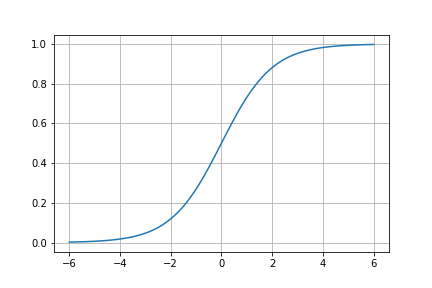
\includegraphics[scale = 0.7]{images/sigmoid.png}
\end{center}
This function has the advantage of being \textbf{derivable}. So, the output of this new  artificial neuron would be:
\[o = \sigma(net) = \frac{1}{1 + e^{-net}}\]
\section{Delta rule}
The \textbf{Delta rule} is a weight update rule different from the Perceptron rule that allows to obtain a best-fit solution approximating the target function. In particular, it exploits \textbf{gradient descent} to explore the hypothesis space and select the hypothesis that best approximates the target function. Its goal is to minimize an error function, appropriately defined.
\subsection{Gradient descent}
\textbf{Derivative:}\newline
The derivative tells us the slope of a function at any point. Given a point:
\begin{itemize}
    \item Positive derivative means that the function increases at that point
    \item Negative derivative means that the function decreases at that point.
    \item Null derivative means that there is a stationary point (minimum, maximum or saddle point).
\end{itemize}
In vector calculus, the gradient of a scalar-valued differentiable function $f: \mathbb{R}^{n} \rightarrow \mathbb{R}$ is a vector-valued function $\nabla f: \mathbb{R}^{n} \rightarrow \mathbb{R}^{n}$ whose value at point $p$ is the vector whose components are the partial derivatives of $f$ at $p$.\newline\newline
The gradient vector can be interpreted as the direction and rate of fastest increase of the function. The gradient is the zero vector at a point if and only if the point is a stationary point.\newline\newline
Let $f(\textbf{x}): \mathbb{R}^{n} \rightarrow \mathbb{R}$ be a vector-valued function, find the vector $\theta \in \mathbb{R}^{n}$ that minimizes the function $f$:
\[\theta = argmin_{\textbf{x}}f(\textbf{x})\]
This minimization problem can be solved using gradient descent. Starting from a random configuration of $\theta$, each parameter is updated in the following way:
\[\theta_{k+1} = \theta_{k} - \eta \nabla f(\theta_{k})\]
where: 
\begin{itemize}
    \item $\nabla f(\theta_{k})$ is the partial derivative of the function in $\theta_{k}$.
    \item The parameter $\eta > 0$ is known as the \textit{learning rate}. 
\end{itemize}
The derivative term $\frac{\partial}{\partial \theta_{k}}f(\theta_{k})$ can be:
\begin{itemize}
    \item $\geq 0$ it means that the function is increasing, so we are decreasing $\theta_{k}$ in the \textit{right direction}.
    \item $\leq 0$ it means that the function is decreasing, so we are increasing $\theta_{k}$ in the \textit{right direction}
\end{itemize}
If $\eta$ is too small, gradient descent can be slow. Anyway, if it is too large, it can overshoot the minimum (fail to converge).\newline\newline
The gradient descent algorithm can be defined as follows:
\begin{enumerate}
    \item $k \leftarrow 0, \theta_{0} \in \mathbb{R}^{n}$
    \item while $\nabla f(\theta_{k}) \neq 0$
    \begin{enumerate}
        \item Compute the descent direction $\textbf{p}_{k} := -\nabla f(\theta_{k})$

        \item Compute the learning rate (fixed) $\eta_{k}$

        \item Update $\theta_{k+1} \leftarrow \theta_{k} + \eta_{k}\textbf{p}_{k}$

        \item $k \leftarrow k + 1$
    \end{enumerate}
\end{enumerate}
The gradient $\nabla f(\theta_{k})$ represents the rate of the fastest increase. So, its opposite represents the direction where the function decreases the most. Note that it is not guaranteed that it converges to a global minimum.
\subsection{Gradient computation (linear activation)}
Consider a Perceptron without the step function \footnote{The step function is not derivable, so we wouldn't be able to compute the gradient} (linear activation).
\[o(\textbf{x}) = \sum_{i=0}^{n}w_{i}x_{i} = \textbf{w} \cdot \textbf{x}\]
and define a measure of the committed error (e.g. mean squared error) given a specific weight vector $\textbf{w}$:
\[E[\textbf{w}] = \frac{1}{2N} \sum_{(\textbf{x}^{(s)}, t^{(s)}) \in S} (t^{(s)} - o(\textbf{x}^{(s)}))^{2}\]
where $N$ is the cardinality of the training set $S$. We want to minimize $E[\textbf{w}]$ with respect to the parameters $\textbf{w}$ using gradient descent. Let's start with the derivation of the loss function $E[\textbf{w}]$:
\[\frac{\partial E}{\partial w_{i}} = \frac{\partial}{\partial w_{i}}\left[\frac{1}{2N}\sum_{s=1}^{N}(t^{(s)} - o^{(s)})^{2} \right]\]
\[= \frac{1}{2N} \sum_{s=1}^{N}\frac{\partial}{\partial w_{i}}\left[ (t^{(s)} - o^{(s)})^{2} \right]\]
\[= \frac{1}{2N}\sum_{s=1}^{N}2(t^{(s)} - o^{(s)})\frac{\partial}{\partial w_{i}}\left[ t^{(s)} - o^{(s)}\right]\]
Note that $t^{(s)}$, which is the target value, is a constant that does not depend on $w_{i}$. So, it can be removed from the derivation.
\[= \frac{1}{N} \sum_{s=1}^{N}(t^{(s)} - o^{(s)})\left(-\frac{\partial}{\partial w_{i}}\left[\textbf{w} \cdot \textbf{x}^{(s)}\right]\right)\]
$\textbf{w} \cdot \textbf{x}^{(s)}$ = $w_{1}x_{1}^{(s)} + w_{2}x_{2}^{(s)} + ... + w_{i}x_{i}^{(s)} + ...$. The partial derivative $-\frac{\partial}{\partial w_{i}}\left[\textbf{w} \cdot \textbf{x}^{(s)}\right]$ with respect to  $w_{i}$ is equal to $x_{i}^{(s)}$ because all the other terms are constant. Therefore, the derivation becomes:
\[ = -\frac{1}{N}\sum_{s=1}^{N}(t^{(s)} - o^{(s)})x_{i}^{(s)}\]
The learning algorithm with gradient descent is defined as follows:\newline\newline
\textbf{Gradient-Descent$(S,\eta)$}:\newline
$\eta$ is the learning rate (that encompasses the constant term $1/N$)
\begin{enumerate}
    \item Initialize the weights $w_{i}$'s with \textbf{small} random values
    \item Repeat until the termination condition is met:
    \begin{enumerate}
        \item $\Delta w_{i} \leftarrow 0$
        \item For each $(\textbf{x},t) \in S$:
        \begin{enumerate}
            \item Compute the output of the neuron $o(\textbf{x}) = \textbf{w} \cdot \textbf{x}$
            \item For each $i \in \{1,...,n\}$
            \[\Delta w_{i} \leftarrow \Delta w_{i} + \eta (t - o)x_{i}\]
        \end{enumerate}
        \item For each $i \in \{1,...,n\}$:
        \[w_{i} \leftarrow w_{i} + \Delta w_{i}\]
    \end{enumerate}
\end{enumerate}
Note that we update the weights using the $+$ because the derivative of the loss function has a $-$ in front of it (so we need to change the sign).
\begin{flushleft}
    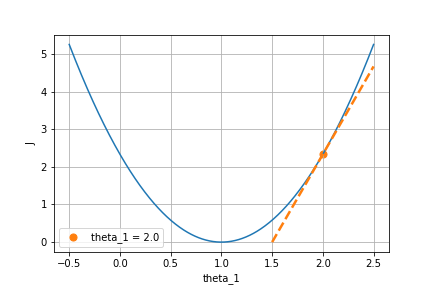
\includegraphics[scale=0.5]{images/partial derivative.png}
    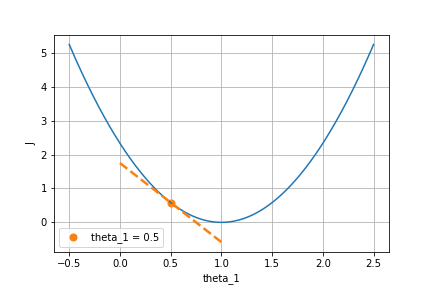
\includegraphics[scale=0.5]{images/partial derivative_1.png}
\end{flushleft}
\begin{center}
    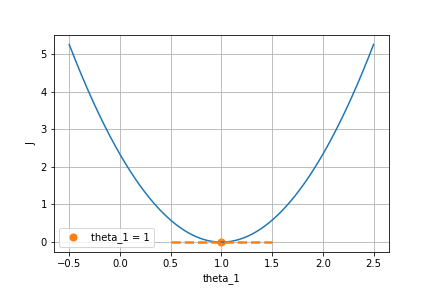
\includegraphics[scale=0.5]{images/partial derivative_2.png}
\end{center}
The graphs above show that this error function has a \textbf{convex} shape (the same is also valid in more than 2 dimensions). This implies that there is a unique global minimum. 
\subsection{Gradient computation (sigmoidal activation)}
Consider now a Perceptron with sigmoidal activation function:
\[o(\textbf{x}) = \sigma \left( \sum_{i=0}^{n}w_{i}x_{i}\right) = \sigma(\textbf{w} \cdot \textbf{x}) = \sigma(y)\]
where $y = \textbf{w} \cdot \textbf{x}$ and $\sigma(y) = \frac{1}{1 + e^{-y}}$. Following the same approach as before, we want to find the weight vector that minimizes the mean squared error in the training set using a gradient descent based algorithm.\newline\newline
The partial derivative of the error function with respect to $w_{i}$ is defined as follows:
\[\frac{\partial E}{\partial w_{i}} = -\frac{1}{N}\sum_{s=1}^{N}(t^{(s)} - o^{(s)})\sigma(y^{(s)})(1 - \sigma(y^{(s)}))x_{i}^{(s)}\]
Hence, the point 2.b.ii of the algorithm presented above becomes:
\[\Delta w_{i} \leftarrow \Delta w_{i} + \eta (t - o)\sigma(y)(1 - \sigma(y))x_{i}\]
Although the sigmoid function is a non-linear function, the Perceptron artificial neuron with sigmoidal activation is still a linear model, because it still produces an hyperplane that separates data.\newline\newline
\textbf{Example:}\newline
In the case of binary classification, given the output of the Perceptron $o^{(s)}$, we can choose to predict the class $y$ of a given instance in the following way:
\begin{itemize}
    \item $y = 1$ if $o^{(s)} \geq 0.5$
    \item $y = 0$ if $o^{(s)} < 0.5$ 
\end{itemize}
For multi-class classification we can use other methods such as the soft-max function.
